\chapter{Fundamentação Teórica} \label{cap:fundamentacao}

Esta seção é dedicada à exploração e discussão dos conceitos e teorias que embasam este trabalho. Neste capítulo, serão apresentados os principais temas e tecnologias envolvidos, como HTTP, NodeJS, \textit{websockets}, e APIs. A discussão será organizada de maneira progressiva, começando pelos conceitos mais gerais e avançando para os aspectos mais específicos e técnicos, como as bibliotecas e \textit{frameworks} utilizados.

\section{Automação de Serviços}

Automação de processos, se refere ao uso de tecnologia para realizar tarefas rotineiras e repetitivas de maneira eficiente e sem erros, e é um aspecto fundamental da automação de serviços.

A automação de serviços é uma tendência em crescimento nos últimos anos, especialmente na área de comércio eletrônico. Ela busca tornar processos mais eficientes, reduzir custos e oferecer melhores experiências aos clientes. Através da automatização, é possível reduzir erros e aumentar a precisão e rapidez no atendimento ao cliente. Com isso, os estabelecimentos podem oferecer um serviço de qualidade, com maior agilidade e menor tempo de espera.

A pandemia de COVID-19 acelerou a necessidade de digitalização em muitos setores. Com as restrições de movimento e o fechamento de lojas físicas, muitos negócios tiveram que se adaptar rapidamente para oferecer seus serviços online. Isso levou a um aumento na demanda por automação de serviços, à medida que as empresas procuravam maneiras de continuar operando de forma eficiente em um ambiente digital. De acordo com um estudo de Sousa, Silva e Araújo (2008), a automação não é apenas uma parte do processo; é um ecossistema em desenvolvimento em que a \glsxtrfull{IA} e a \gls{IoT} trabalham juntas para criar uma força de trabalho mais inteligente, eficiente e produtiva \cite{Gourley2002}.


\section{Comunicação HTTP e Web} \label{sec:http}

O protocolo \glsxtrfull{HTTP} é um dos principais métodos para transferência de dados via \textit{web}. Trata-se de um protocolo de cliente-servidor, o que significa que as solicitações são iniciadas pelo cliente, geralmente o navegador da \textit{web}, e um documento completo é reconstruído a partir dos diferentes recursos buscados, como texto, descrição de \textit{layout}, imagens, vídeos, \textit{scripts} e mais \cite{mdn_http_overview}, a Figura \ref{fig:http-get} ilustra esse processo.

\begin{figure}[h]
\centering
\caption{Buscando dados da Web.}
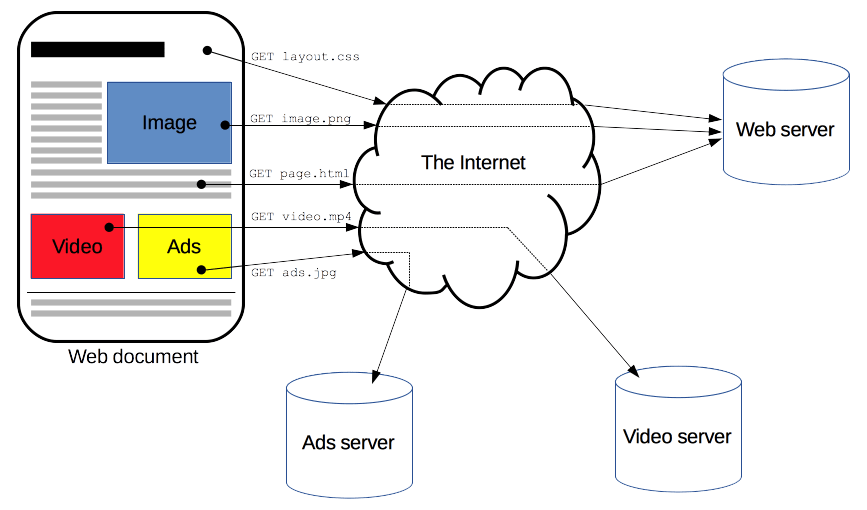
\includegraphics[width=0.8\textwidth]{figuras/fetching_a_page.png}
\fonte{\cite{mdn_http_overview}.}
\label{fig:http-get}
\end{figure}

O \gls{HTTP} é um protocolo sem estado, o que significa que cada requisição é independente das outras. Isso permite que a web seja altamente escalável, pois os servidores não precisam manter informações sobre cada usuário.

A \gls{WWW} foi criada em 1989 por Tim Berners-Lee, um cientista da computação britânico que trabalhava no CERN, o laboratório de física de partículas na Suíça. O objetivo era criar uma maneira fácil de compartilhar informações entre os cientistas que trabalhavam em diferentes universidades e institutos ao redor do mundo. O \gls{HTML} foi a linguagem de marcação que Berners-Lee desenvolveu para criar páginas \textit{web}. A Figura \ref{fig:http-html} demonstra a conexão entre estas tecnologias e como elas se encaixam para produzir a \textit{web}.

\begin{figure}[h]
\centering
\caption{Camadas da \textit{web}.}
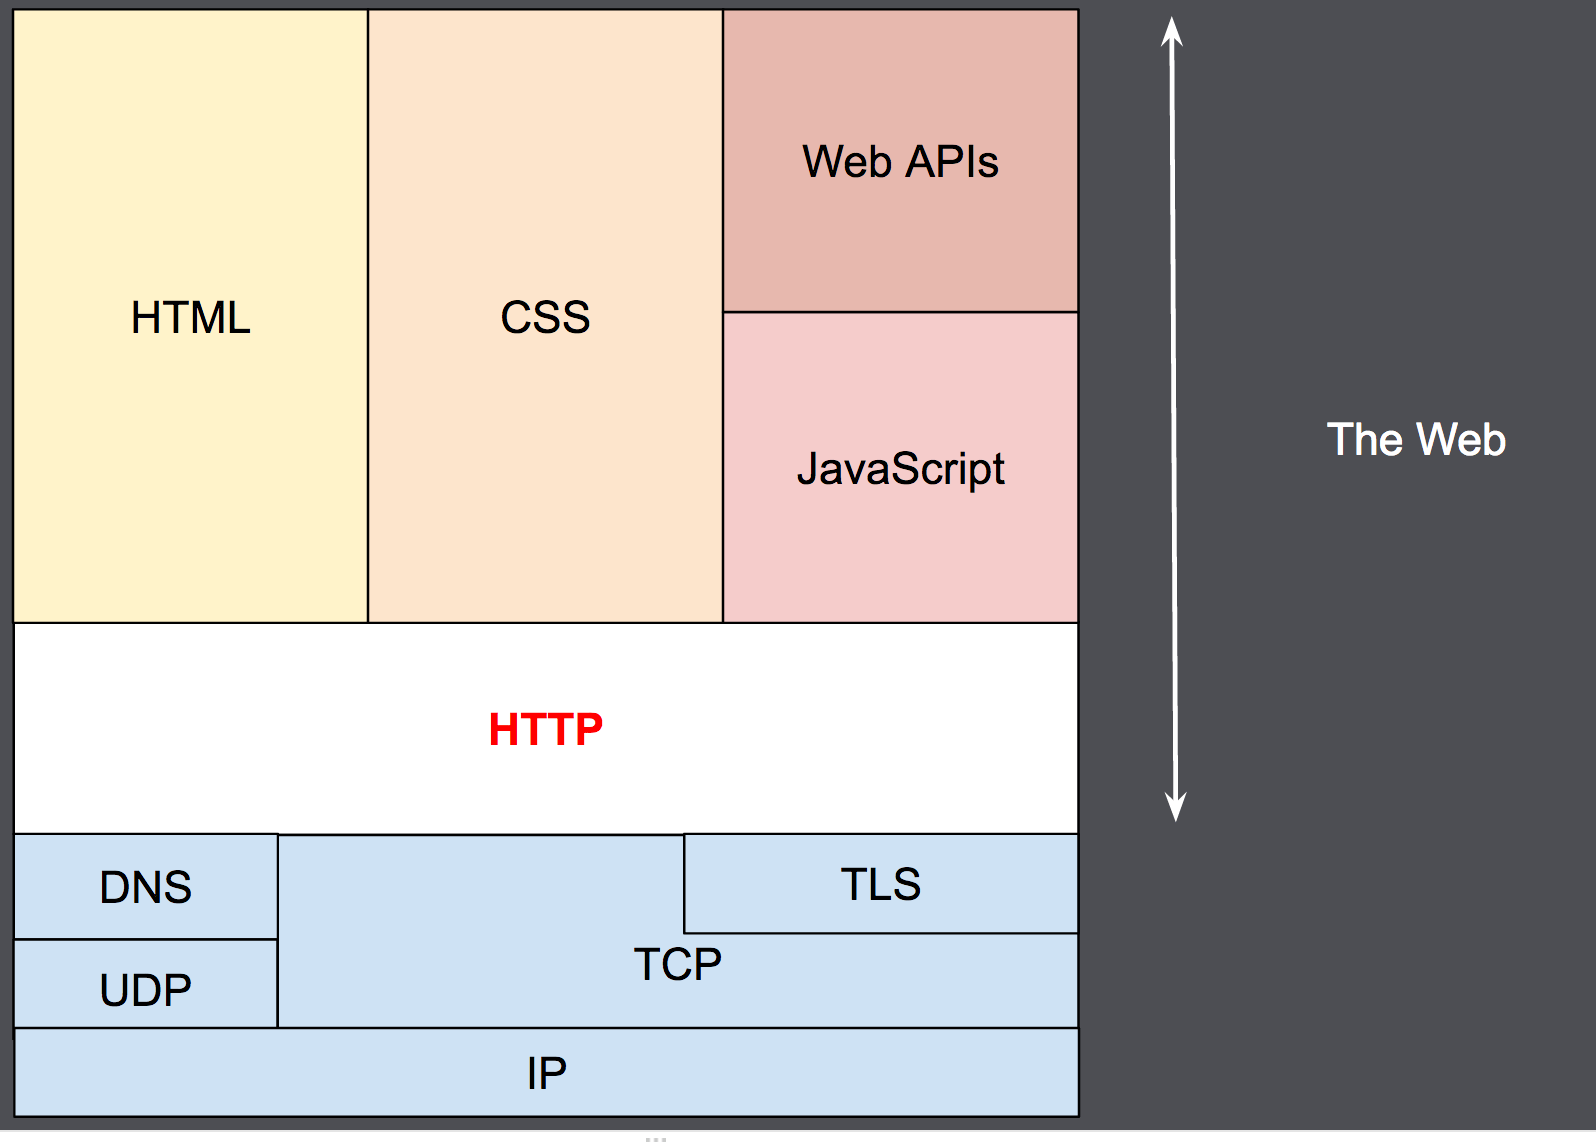
\includegraphics[width=0.8\textwidth]{figuras/http-layers.png}
\fonte{\cite{mdn_http_overview}.}
\label{fig:http-html}
\end{figure}

Com o tempo, o \gls{HTTP} evoluiu e novas versões foram lançadas. A versão mais recente é o \gls{HTTP}/3, que oferece melhor desempenho e segurança em comparação com as versões anteriores. No entanto, o \gls{HTTP}/1.1 e \gls{HTTP}/2 ainda são amplamente utilizados na \textit{web} \cite{HttpIEEE}.

Um conceito importante para a comunicação HTTP são os métodos, os principais métodos HTTP são:

\begin{itemize}
\item \textbf{GET:} Solicita um recurso do servidor. Este é o método mais comum e é usado para solicitar a visualização de páginas da web.
\item \textbf{POST:} Envia dados para o servidor para criar um novo recurso. Os dados são incluídos no corpo da solicitação.
\item \textbf{PUT:} Envia dados para o servidor para atualizar um recurso existente. Os dados são incluídos no corpo da solicitação.
\item \textbf{DELETE:} Solicita a exclusão de um recurso no servidor.
\item \textbf{OPTIONS:} Solicita informações sobre os métodos de comunicação disponíveis para um recurso ou para o servidor em geral.
\item \textbf{PATCH:} Aplica modificações parciais a um recurso.
\item \textbf{CONNECT:} É usado para abrir uma conexão de rede bidirecional com o recurso solicitado. Geralmente é usado para acesso SSL (HTTPS).
\end{itemize}

Esses métodos são definidos no protocolo HTTP e são usados para indicar a ação desejada a ser realizada no recurso especificado. Eles formam a base da interação entre o cliente e o servidor na web \cite{HttpIEEE}.

\section{API}

Uma \glsxtrfull{API} é um conjunto de rotinas, protocolos e ferramentas para construção de software e aplicações. Ela define como os componentes de software devem interagir entre si, permitindo que diferentes aplicações possam se comunicar e compartilhar informações \cite{Mulloy2012}.

\subsection{REST API}

\glsxtrfull{REST} é um estilo arquitetural para sistemas distribuídos, baseado no protocolo HTTP. Ele define um conjunto de restrições que devem ser seguidas para que as aplicações possam se comunicar de forma eficiente e escalável. Uma das principais características do REST é a separação entre cliente e servidor, onde o cliente faz requisições ao servidor para acessar recursos, e o servidor responde com uma representação do estado atual do recurso solicitado. A Figura \ref{fig:rest} mostra a arquitetura de uma REST API.

\begin{figure}[h]
\centering
\caption{API Rest.}
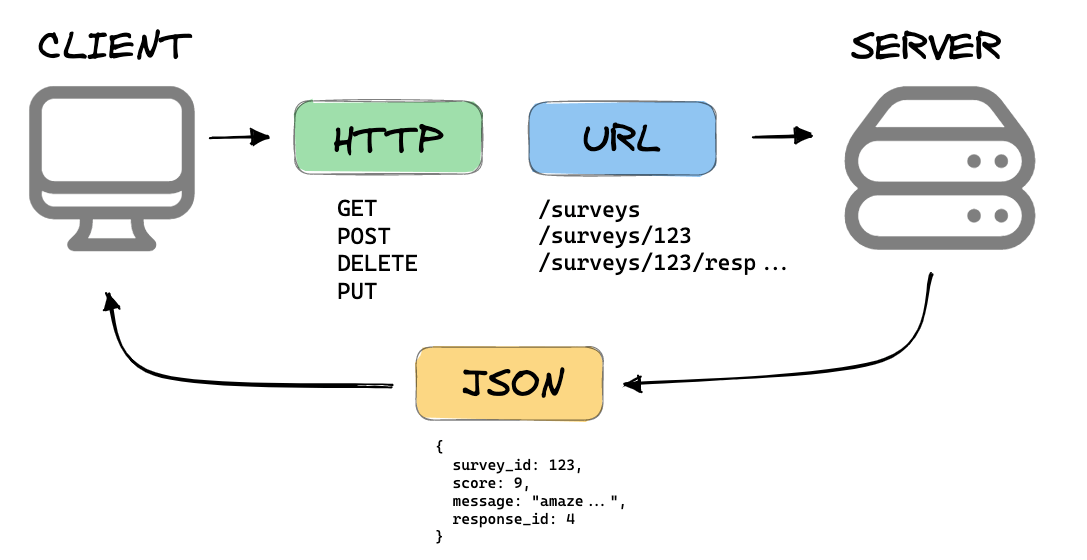
\includegraphics[width=0.8\textwidth]{figuras/rest-api.png}
\fonte{\cite{restAPI}.}
\label{fig:rest}
\end{figure}

O \gls{REST} é um elemento fundamental na construção de APIs modernas, devido à sua simplicidade e eficiência. Ele permite que os desenvolvedores criem APIs que podem ser facilmente consumidas por diferentes clientes, incluindo navegadores web, aplicativos móveis e outros servidores. Além disso, o \gls{REST} é independente de linguagem, o que significa que pode ser usado com qualquer linguagem de programação que suporte \gls{HTTP}.

O \gls{REST} foi proposto por Roy Fielding em sua tese de doutorado em 2000. Fielding é um dos principais contribuidores para o desenvolvimento do protocolo HTTP e co-fundador da Apache \gls{HTTP} Server Project. Em sua tese, Fielding descreveu o REST como um conjunto de princípios arquiteturais que podem ser usados para projetar sistemas distribuídos que são escaláveis, eficientes e fáceis de modificar e manter.

Os métodos HTTP citados na Seção \ref{sec:http} são incorporados ao REST. Eles formam um estilo arquitetural que utiliza métodos com a mesma semântica para permitir a construção de APIS, com rotas do tipo POST, GET, DELETE etc.

Desde então, o \gls{REST} se tornou o estilo arquitetural mais popular para a construção de APIs na web. Ele é usado por muitas grandes empresas, incluindo Google, Facebook e Twitter, para fornecer acesso programático aos seus serviços \cite{Richardson2007}.

\subsection{APIs de Pagamento}

As \gls{API}s de pagamento surgiram como uma necessidade para facilitar as transações online. No início, as APIs de pagamento eram principalmente usadas para processar pagamentos com cartão de crédito. Empresas como a PayPal foram pioneiras nesse campo, fornecendo APIs que permitiam aos comerciantes aceitar pagamentos com cartão de crédito em seus sites.

Com o tempo, as APIs de pagamento evoluíram para suportar uma variedade de métodos de pagamento. Isso inclui não apenas cartões de crédito, mas também débito direto, pagamentos móveis e até mesmo cripto-moedas. Além disso, as APIs de pagamento também começaram a oferecer funcionalidades adicionais, como suporte para pagamentos recorrentes, reembolsos, e a capacidade de gerenciar várias moedas.

No Brasil, intermediários de pagamento como o Mercado Pago e o PagSeguro oferecem APIs que permitem aos comerciantes aceitar uma variedade de métodos de pagamento, incluindo boleto bancário e transferências bancárias. Recentemente, com a introdução do PIX, um sistema de pagamentos instantâneos operado pelo Banco Central do Brasil, esses intermediários também começaram a oferecer APIs que suportam PIX, permitindo transações quase instantâneas \cite{Aue2018, Adyen}.

\section{Sockets e WebSockets}
Os \textit{sockets e webSockets} são tecnologias fundamentais para a comunicação em tempo real na internet. \textit{Sockets} são um mecanismo de comunicação bidirecional entre dois nós em uma rede, permitindo a troca de dados em tempo real. Eles são amplamente utilizados em sistemas distribuídos e aplicações de rede para estabelecer conexões entre servidores e clientes \cite{Attoui2000}.

Os \textit{websockets}, por outro lado, são uma extensão dos \textit{sockets}, projetados especificamente para comunicação em tempo real na web. Eles superam as limitações das soluções tradicionais de comunicação em tempo real na web, como \textit{polling e long-polling}, fornecendo um mecanismo eficaz para comunicação bidirecional sustentada entre o cliente e o servidor. A tecnologia \textit{websockets} permite uma comunicação mais eficiente, reduzindo o tráfego de rede e a latência, tornando-a ideal para aplicações que exigem interações em tempo real \cite{Liu2012}.

\section{Tokens e JWT}

A autenticação e a autorização são componentes críticos de qualquer aplicação segura. \textit{Tokens}, particularmente \glsxtrfull{JWT}, são usados para transmitir informações de forma segura entre partes. \gls{JWT} é um padrão aberto (RFC 7519) que define uma maneira compacta e independente de transmitir informações entre partes como um \gls{JSON}. Essas informações podem ser verificadas e confiáveis porque são assinadas digitalmente. JWT pode ser assinado usando um segredo (com o algoritmo HMAC) ou um par de chaves pública/privada usando RSA ou ECDSA \cite{JWT2023}.

\section{QR Code}

O código \glsxtrfull{QR} é um código de barras bidimensional que pode armazenar informações em um formato legível por máquina. Ele foi desenvolvido para permitir a leitura rápida e eficiente de informações por dispositivos eletrônicos, como \textit{smartphones e tablets}.

Amplamente utilizado em várias aplicações, o QR Code se tornou muito comum no rastreamento de produtos, gerenciamento de inventário e marketing \cite{QRCode2023}. A Figura \ref{fig:qr} demonstra um QR que foi gerado com um \textit{link}.

\begin{figure}[h]
\centering
\caption{QR Code com link para loja.}

\includegraphics[width=0.4\textwidth]{figuras/qr.png}
\fonte{Criado pelo autor.}
\label{fig:qr}
\end{figure}

Esta codificação é gerada através de um processo que transforma a informação desejada (como um \textit{link} para um site) em um padrão de pontos pretos e brancos. Este padrão é lido por um \textit{scanner} (geralmente uma câmera de \textit{smartphones} com um aplicativo de leitura de QR Code), que decodifica a informação e realiza a ação correspondente (como abrir um \textit{link} em um navegador).

\section{Internet das Coisas (IoT)}
\gls{IoT} é discutido como uma tecnologia emergente que transforma objetos do mundo real em objetos virtuais inteligentes. \gls{IoT} visa unificar tudo em nosso mundo sob uma infraestrutura comum, não apenas nos dando controle sobre as coisas ao nosso redor, mas também nos mantendo informados sobre o estado dessas coisas \cite{Madakam:2015}. 

Isso torna possível a criação de dispositivos conectados a internet, capazes de monitorar e controlar processos e equipamentos remotamente. \gls{IoT} tem um papel crucial na transformação digital e na criação de cidades inteligentes, permitindo a coleta de dados em tempo real e a tomada de decisões baseada em dados. A Figura \ref{fig:iot} representa como diversos dispositivos se conectam a internet através da IoT.

\begin{figure}[h]
\centering
\caption{Internet of Things.}
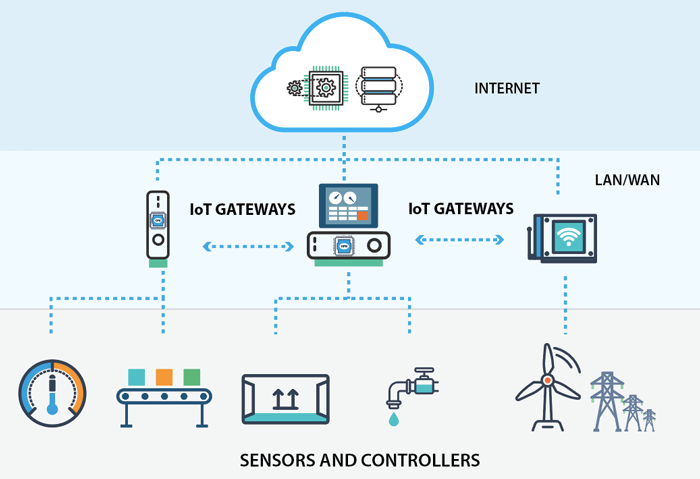
\includegraphics[width=0.8\textwidth]{figuras/iot.png}
\fonte{\cite{iot123}.}
\label{fig:iot}
\end{figure}

\section{UUID}

Um \glsxtrfull{UUID} é um identificador único de 128 bits que é usado para identificar informações de forma única em um sistema de computação distribuído \cite{Leach2005}. Ele é gerado de forma aleatória, tornando-o altamente improvável de ser duplicado. O formato de UUID mais comum é o \gls{UUID} versão 4, que utiliza a geração aleatória de números para criar uma identificação única. O UUID é amplamente utilizado em sistemas distribuídos, como bancos de dados, sistemas de mensagens e sistemas de arquivos distribuídos \cite{Leach2005}.

Essa ferramenta permite que cada elemento seja rastreado e gerenciado de forma única, evitando conflitos ou duplicatas no sistema. Além disso, aumenta a segurança, visto que dificulta tentativas, por parte de usuários mal intencionados, de manipular algum elemento do sistema.

\section{Tecnologias da Aplicação Web}

Neste trabalho, serão utilizadas diversas tecnologias e bibliotecas. As mais importantes são explicadas nas seções a seguir. 

\subsection{TypeScript}

TypeScript é uma linguagem de programação que estende o JavaScript, adicionando tipos estáticos. Sua principal motivação é permitir o desenvolvimento de aplicações JavaScript em larga escala de maneira mais eficiente. O TypeScript introduz um sistema de módulos, classes e interfaces, além de um sistema de tipos gradual e robusto. Essas características permitem que os desenvolvedores escrevam código JavaScript de maneira mais clara e estruturada, facilitando a compreensão e a manutenção do código \cite[p.~257]{Bierman:2014}.

O TypeScript oferece ferramentas que auxiliam na construção do código, como a capacidade de listar os campos presentes em um objeto ou todos os métodos de uma classe. Isso facilita a navegação e a manipulação do código, especialmente em projetos de grande escala. Além disso, o TypeScript, por meio de seu sistema de tipos estáticos, é capaz de fornecer garantias sobre o comportamento do código, assegurando que os tipos de dados sejam consistentes ao longo do código, o que pode resultar em software mais confiável e de maior qualidade. Essas características tornam o TypeScript uma escolha popular para o desenvolvimento de aplicações web de grande escala, tanto para front-end quanto para back-end.

\subsection{SQL e Prisma}

\glsxtrfull{SQL} é uma linguagem de programação utilizada para gerenciar e manipular bancos de dados. Ela permite aos usuários criar, ler, atualizar e deletar dados em um banco de dados. SQL é uma linguagem padrão para bancos de dados relacionais e é usada em muitos sistemas de gerenciamento de bancos de dados, como MySQL, Oracle, PostgreSQL e SQL Server. SQL é uma linguagem essencial para desenvolvedores de software, analistas de dados e administradores de banco de dados, pois permite a interação eficiente com os dados armazenados em um banco de dados~\cite{SQL2023}.

No entanto, trabalhar diretamente com SQL pode ser complexo e propenso a erros. Para resolver isso, os desenvolvedores usam ferramentas chamadas mapeadores objeto-relacional (ORMs). Um ORM permite que os desenvolvedores interajam com o banco de dados usando o paradigma de programação orientada a objetos, o que é mais intuitivo e seguro para muitos desenvolvedores.

O Prisma é um ORM moderno e poderoso que permite o acesso a bancos de dados através de uma interface simples e intuitiva. Ele oferece diversas funcionalidades, como migrações de banco de dados, controle de versão de esquema e consultas otimizadas, permitindo um acesso rápido e eficiente aos dados. O Prisma pode ser usado para acessar bancos de dados de forma eficiente e segura, com suporte para várias funcionalidades, como migrações automáticas, cliente de banco de dados com tipagem segura e navegador de banco de dados visual \cite{Prisma2023}.

\subsection{Zod}

Zod é uma biblioteca para TypeScript que ajuda a garantir que os dados em uma aplicação estejam corretos e seguros. Ele faz isso através do uso de "esquemas", que são como modelos que descrevem como os dados devem ser estruturados, incluindo o tipo de dados e regras. Por exemplo, um esquema pode especificar que um item em uma loja online deve ter um nome (caracteres), uma descrição (caracteres) e um preço (número). O trecho de Código \ref{code:zod} mostra como esse elemento pode ser representado através dessa biblioteca, criando um tipo de dado chamado ``itemSchema''.

\renewcommand{\lstlistingname}{Código Fonte}

\begin{figure}[h]
\begin{lstlisting}[caption={Exemplo de uso da biblioteca Zod.},label={code:zod}]
import z from 'zod';

export const itemSchema = z.object({
  id: z.string().uuid(),
  name: z.string(),
  description: z.string().min(4),
  price: z.number(),
});
\end{lstlisting}
\fonte{Criado pelo autor.}
\end{figure}

Com Zod, é possível definir esses esquemas e usar a biblioteca para verificar se os dados de entrada e saída da aplicação correspondem a esses esquemas. Isso é especialmente útil em aplicações web, onde os dados de entrada geralmente vêm de usuários e podem ser imprevisíveis.

Ao usar Zod para validar esses dados, é possível prevenir muitos erros e vulnerabilidades de segurança, tornando a aplicação mais robusta e confiável \cite{Zod2023}.

\subsection{tRPC}
O \glsxtrfull{tRPC} é uma biblioteca leve que permite a criação de APIs totalmente seguras em termos de tipo \cite{tRPC}. Ele se apresenta como uma alternativa a outras tecnologias de chamada de procedimento remoto, como REST, GraphQL e gRPC.

Ele permite que os desenvolvedores criem APIs, sem a necessidade de manter manualmente as definições do formato dos dados entre o cliente e o servidor. Isso é conseguido através da geração automática de definições de tipo com base no código do servidor. Em outras palavras, o tRPC entende quais dados devem ser enviados na requisição, com base no código do servidor, eliminando a necessidade de manutenção manual dessas definições \cite{tRPC}. Complementando o que foi exibido anteriormente com o Zod, o Código \ref{code:tRPC} demonstra a implementação de uma rota backend que utiliza tRPC e Zod.

\begin{figure}[h]
\begin{lstlisting}[caption={Exemplo de uso da biblioteca tRPC no backend.},label={code:tRPC}]

export const itemsRouter = createTRPCRouter({
  create: publicProcedure
    .input(
      z.object({
        name: z.string(),
        description: z.string().min(4),
        price: z.number(),
      })
    )
    .mutation(({ ctx, input }) => {
      return ctx.prisma.items.create({
        data: {
          description: input.description,
          price: input.price,
          name: input.name,
        },
      });
    }),
});
\end{lstlisting}
\fonte{Criado pelo autor.}
\end{figure}

O Código \ref{code:trpc2}, corresponde a uma implementação do tRPC no frontend, que utiliza esta rota para enviar informações.

\begin{figure}[h]
\begin{lstlisting}[caption={Exemplo de uso da biblioteca tRPC no frontend.}, label={code:trpc2}]
export const itemsRouter = createTRPCRouter({
   // importa a rota da api trpc
  const createItem = api.items.create.useMutation({
    onSuccess: (createdItem) => {
      toast.success("Item criado com sucesso", {
        position: "top-right",
        autoClose: 3000,
        theme: "colored",
      });
      },
      onError: (err) => {
      toast.error("Erro ao criar item", {
        position: "top-right",
        autoClose: 5000,
        theme: "colored",
      });
      }
    });

    // utilizacao dela para enviar a requisicao
    createItem.mutate({
        name: values.name,
        description: values.description,
        price: values.price,
      });
\end{lstlisting}
\fonte{Criado pelo autor.}
\end{figure}

No contexto de desenvolvimento full stack, o tRPC se destaca como uma biblioteca fundamental para a construção tanto do servidor quanto do cliente. De acordo com o trabalho de \cite{Nivasalo2022}, o tRPC se mostrou uma excelente biblioteca para se basear, pois reduziu significativamente o tempo de desenvolvimento ao tornar extremamente fácil a implementação de chamadas de endpoint da API para o frontend.

Por fim, vale ressaltar que o tRPC é um projeto de código aberto e gratuito para uso, o que o torna uma excelente opção para desenvolvedores e empresas que buscam uma solução eficiente e econômica para a criação de APIs seguras em termos de tipo.

\subsection{Fastify}

Fastify é um \textit{framework} web eficiente para Node.js, projetado para ser o mais rápido possível, tanto em termos de tempo de execução quanto de velocidade de desenvolvimento \cite{fastify}. Ele fornece um conjunto robusto de recursos para construir aplicações web e é totalmente extensível com seu sistema de \textit{plugins}. Fastify também oferece um modelo de roteamento fácil de usar e suporte para manipulação de solicitações e respostas HTTP, tornando-o uma escolha popular para muitos desenvolvedores de Node.js.

\subsection{Next.js}

Next.js é um \textit{framework} JavaScript para sistemas baseados em React, que permite a criação de páginas estáticas e dinâmicas, bem como a geração de conteúdo sob demanda, proporcionando uma experiência de carregamento mais rápida e eficiente para o usuário. Este \textit{framework} pode ser usado para criar aplicações web eficientes e escaláveis, com suporte para várias funcionalidades, como roteamento por arquivo, \textit{streaming} de HTML dinâmico e suporte a CSS \cite{Nextjs2023}.

Amplamente utilizado e reconhecido na indústria de desenvolvimento web, o NextJs é o 14º maior projeto no GitHub e é considerado o \textit{framework} ReactJS número 1, com mais de 100.000 estrelas no GitHub. Grandes empresas como Notion e Twitch utilizam o Next.js em suas aplicações, o que demonstra a confiabilidade e a maturidade do \textit{framework} \cite{Vercel2023}.

Além disso, o Next.js é recomendado na documentação oficial do React para projetos  que se beneficiariam de suas características específicas, como renderização do lado do servidor e otimizações de desempenho. Isso indica a importância e a relevância do Next.js no ecossistema de desenvolvimento web atual. A adoção do Next.js neste trabalho é uma escolha estratégica que visa aproveitar essas vantagens e recursos poderosos para criar uma aplicação web robusta e eficiente.

\section{NodeMCU ESP8266}

O NodeMCU ESP8266 é um microcontrolador baseado na plataforma ESP8266, que possui conectividade Wi-Fi integrada. Ele é bastante utilizado em projetos de \gls{IoT} devido à sua facilidade de programação, baixo custo e recursos avançados. O ESP8266, demonstrado na Figura \ref{fig:node}, é especialmente adequado para tais aplicações devido à sua capacidade de operar em baixa potência, o que é crucial para dispositivos alimentados por bateria, e sua capacidade de se conectar a redes Wi-Fi, permitindo a comunicação com a internet e outros dispositivos na rede  \cite{Kolban2016}.

\begin{figure}[h]
\centering
\caption{ESP8266 NodeMcu.}
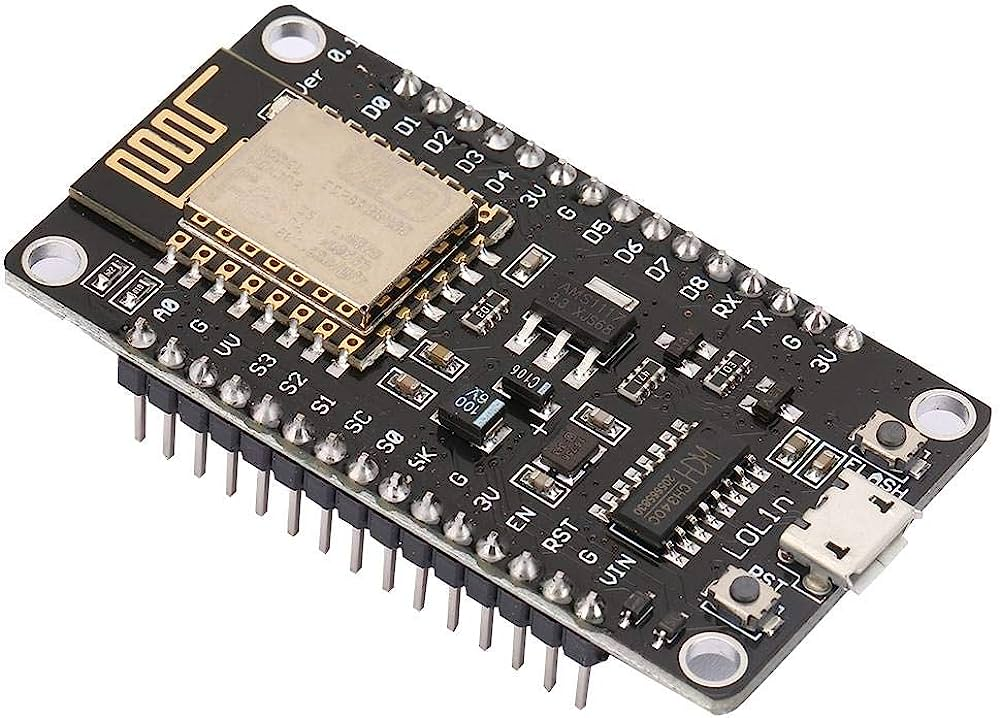
\includegraphics[width=0.5\textwidth]{figuras/nodemcu.jpg}
\fonte{\cite{nodemcu}.}
\label{fig:node}
\end{figure}

\subsection{C++ e Bibliotecas}

O microcontrolador NodeMCU, pode ser programado em C++ e as bibliotecas relevantes para este projeto estão listadas a seguir.
\begin{itemize}
\item \textbf{ESP8266WiFi.h:} Esta biblioteca permite que o NodeMCU se conecte a redes Wi-Fi. Ela fornece funções para conectar, desconectar e verificar o status da conexão WiFi. No código fornecido, essa biblioteca é usada para conectar o NodeMCU à rede Wi-Fi especificada pelas constantes ``ssid'' e ``password''.

\item \textbf{WebSocketsClient.h:} Esta biblioteca permite que o NodeMCU se comunique com servidores \textit{websocket}. \textit{Websocket} é um protocolo que permite comunicação bidirecional em tempo real entre clientes e servidores. No código fornecido, essa biblioteca é usada para conectar o NodeMCU a um servidor \textit{websocket} e enviar/receber mensagens.
\end{itemize}


% ----------------------------------------------------------



